% Included by sections/04-dataset.tex. Regenerate with
%   node workspace/figures/make_difficulty_grid_figure.mjs
% then copy workspace/figures/out/difficulty_grid.tex here and drop the standalone wrapper.
\begin{figure}[t]
\centering
% Corpus coverage over fold depth and coupling.
% Generated by workspace/figures/make_difficulty_grid_figure.mjs
% Source: /Users/luxian/FoldOriganmi/workspace/corpus/out/release (600 samples, peak cell 54)
%
% Standalone: pdflatex difficulty_grid.tex
% In a paper: keep the tikzpicture, drop the documentclass wrapper.
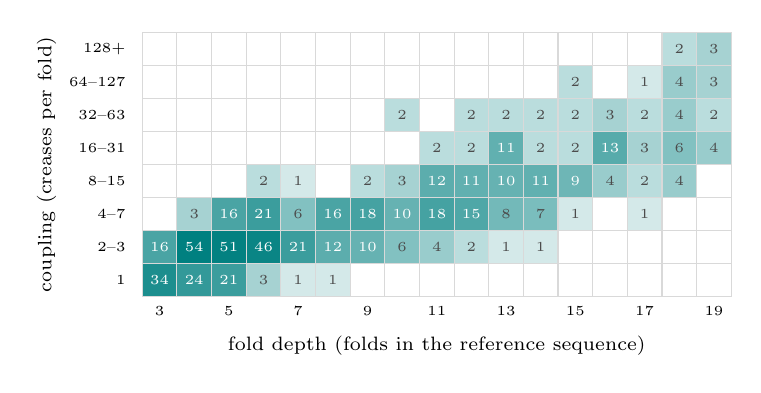
\begin{tikzpicture}[x=0.44cm, y=0.42cm, font=\scriptsize]
\fill[teal!89!white] (0,0) rectangle ++(1,1); \draw[gray!30] (0,0) rectangle ++(1,1); \node[font=\tiny, white] at (0.5,0.5) {34};
\fill[teal!80!white] (1,0) rectangle ++(1,1); \draw[gray!30] (1,0) rectangle ++(1,1); \node[font=\tiny, white] at (1.5,0.5) {24};
\fill[teal!77!white] (2,0) rectangle ++(1,1); \draw[gray!30] (2,0) rectangle ++(1,1); \node[font=\tiny, white] at (2.5,0.5) {21};
\fill[teal!35!white] (3,0) rectangle ++(1,1); \draw[gray!30] (3,0) rectangle ++(1,1); \node[font=\tiny, black!70] at (3.5,0.5) {3};
\fill[teal!17!white] (4,0) rectangle ++(1,1); \draw[gray!30] (4,0) rectangle ++(1,1); \node[font=\tiny, black!70] at (4.5,0.5) {1};
\fill[teal!17!white] (5,0) rectangle ++(1,1); \draw[gray!30] (5,0) rectangle ++(1,1); \node[font=\tiny, black!70] at (5.5,0.5) {1};
\draw[gray!30] (6,0) rectangle ++(1,1);
\draw[gray!30] (7,0) rectangle ++(1,1);
\draw[gray!30] (8,0) rectangle ++(1,1);
\draw[gray!30] (9,0) rectangle ++(1,1);
\draw[gray!30] (10,0) rectangle ++(1,1);
\draw[gray!30] (11,0) rectangle ++(1,1);
\draw[gray!30] (12,0) rectangle ++(1,1);
\draw[gray!30] (13,0) rectangle ++(1,1);
\draw[gray!30] (14,0) rectangle ++(1,1);
\draw[gray!30] (15,0) rectangle ++(1,1);
\draw[gray!30] (16,0) rectangle ++(1,1);
\fill[teal!71!white] (0,1) rectangle ++(1,1); \draw[gray!30] (0,1) rectangle ++(1,1); \node[font=\tiny, white] at (0.5,1.5) {16};
\fill[teal!100!white] (1,1) rectangle ++(1,1); \draw[gray!30] (1,1) rectangle ++(1,1); \node[font=\tiny, white] at (1.5,1.5) {54};
\fill[teal!99!white] (2,1) rectangle ++(1,1); \draw[gray!30] (2,1) rectangle ++(1,1); \node[font=\tiny, white] at (2.5,1.5) {51};
\fill[teal!96!white] (3,1) rectangle ++(1,1); \draw[gray!30] (3,1) rectangle ++(1,1); \node[font=\tiny, white] at (3.5,1.5) {46};
\fill[teal!77!white] (4,1) rectangle ++(1,1); \draw[gray!30] (4,1) rectangle ++(1,1); \node[font=\tiny, white] at (4.5,1.5) {21};
\fill[teal!64!white] (5,1) rectangle ++(1,1); \draw[gray!30] (5,1) rectangle ++(1,1); \node[font=\tiny, white] at (5.5,1.5) {12};
\fill[teal!60!white] (6,1) rectangle ++(1,1); \draw[gray!30] (6,1) rectangle ++(1,1); \node[font=\tiny, white] at (6.5,1.5) {10};
\fill[teal!49!white] (7,1) rectangle ++(1,1); \draw[gray!30] (7,1) rectangle ++(1,1); \node[font=\tiny, black!70] at (7.5,1.5) {6};
\fill[teal!40!white] (8,1) rectangle ++(1,1); \draw[gray!30] (8,1) rectangle ++(1,1); \node[font=\tiny, black!70] at (8.5,1.5) {4};
\fill[teal!27!white] (9,1) rectangle ++(1,1); \draw[gray!30] (9,1) rectangle ++(1,1); \node[font=\tiny, black!70] at (9.5,1.5) {2};
\fill[teal!17!white] (10,1) rectangle ++(1,1); \draw[gray!30] (10,1) rectangle ++(1,1); \node[font=\tiny, black!70] at (10.5,1.5) {1};
\fill[teal!17!white] (11,1) rectangle ++(1,1); \draw[gray!30] (11,1) rectangle ++(1,1); \node[font=\tiny, black!70] at (11.5,1.5) {1};
\draw[gray!30] (12,1) rectangle ++(1,1);
\draw[gray!30] (13,1) rectangle ++(1,1);
\draw[gray!30] (14,1) rectangle ++(1,1);
\draw[gray!30] (15,1) rectangle ++(1,1);
\draw[gray!30] (16,1) rectangle ++(1,1);
\draw[gray!30] (0,2) rectangle ++(1,1);
\fill[teal!35!white] (1,2) rectangle ++(1,1); \draw[gray!30] (1,2) rectangle ++(1,1); \node[font=\tiny, black!70] at (1.5,2.5) {3};
\fill[teal!71!white] (2,2) rectangle ++(1,1); \draw[gray!30] (2,2) rectangle ++(1,1); \node[font=\tiny, white] at (2.5,2.5) {16};
\fill[teal!77!white] (3,2) rectangle ++(1,1); \draw[gray!30] (3,2) rectangle ++(1,1); \node[font=\tiny, white] at (3.5,2.5) {21};
\fill[teal!49!white] (4,2) rectangle ++(1,1); \draw[gray!30] (4,2) rectangle ++(1,1); \node[font=\tiny, black!70] at (4.5,2.5) {6};
\fill[teal!71!white] (5,2) rectangle ++(1,1); \draw[gray!30] (5,2) rectangle ++(1,1); \node[font=\tiny, white] at (5.5,2.5) {16};
\fill[teal!73!white] (6,2) rectangle ++(1,1); \draw[gray!30] (6,2) rectangle ++(1,1); \node[font=\tiny, white] at (6.5,2.5) {18};
\fill[teal!60!white] (7,2) rectangle ++(1,1); \draw[gray!30] (7,2) rectangle ++(1,1); \node[font=\tiny, white] at (7.5,2.5) {10};
\fill[teal!73!white] (8,2) rectangle ++(1,1); \draw[gray!30] (8,2) rectangle ++(1,1); \node[font=\tiny, white] at (8.5,2.5) {18};
\fill[teal!69!white] (9,2) rectangle ++(1,1); \draw[gray!30] (9,2) rectangle ++(1,1); \node[font=\tiny, white] at (9.5,2.5) {15};
\fill[teal!55!white] (10,2) rectangle ++(1,1); \draw[gray!30] (10,2) rectangle ++(1,1); \node[font=\tiny, black!70] at (10.5,2.5) {8};
\fill[teal!52!white] (11,2) rectangle ++(1,1); \draw[gray!30] (11,2) rectangle ++(1,1); \node[font=\tiny, black!70] at (11.5,2.5) {7};
\fill[teal!17!white] (12,2) rectangle ++(1,1); \draw[gray!30] (12,2) rectangle ++(1,1); \node[font=\tiny, black!70] at (12.5,2.5) {1};
\draw[gray!30] (13,2) rectangle ++(1,1);
\fill[teal!17!white] (14,2) rectangle ++(1,1); \draw[gray!30] (14,2) rectangle ++(1,1); \node[font=\tiny, black!70] at (14.5,2.5) {1};
\draw[gray!30] (15,2) rectangle ++(1,1);
\draw[gray!30] (16,2) rectangle ++(1,1);
\draw[gray!30] (0,3) rectangle ++(1,1);
\draw[gray!30] (1,3) rectangle ++(1,1);
\draw[gray!30] (2,3) rectangle ++(1,1);
\fill[teal!27!white] (3,3) rectangle ++(1,1); \draw[gray!30] (3,3) rectangle ++(1,1); \node[font=\tiny, black!70] at (3.5,3.5) {2};
\fill[teal!17!white] (4,3) rectangle ++(1,1); \draw[gray!30] (4,3) rectangle ++(1,1); \node[font=\tiny, black!70] at (4.5,3.5) {1};
\draw[gray!30] (5,3) rectangle ++(1,1);
\fill[teal!27!white] (6,3) rectangle ++(1,1); \draw[gray!30] (6,3) rectangle ++(1,1); \node[font=\tiny, black!70] at (6.5,3.5) {2};
\fill[teal!35!white] (7,3) rectangle ++(1,1); \draw[gray!30] (7,3) rectangle ++(1,1); \node[font=\tiny, black!70] at (7.5,3.5) {3};
\fill[teal!64!white] (8,3) rectangle ++(1,1); \draw[gray!30] (8,3) rectangle ++(1,1); \node[font=\tiny, white] at (8.5,3.5) {12};
\fill[teal!62!white] (9,3) rectangle ++(1,1); \draw[gray!30] (9,3) rectangle ++(1,1); \node[font=\tiny, white] at (9.5,3.5) {11};
\fill[teal!60!white] (10,3) rectangle ++(1,1); \draw[gray!30] (10,3) rectangle ++(1,1); \node[font=\tiny, white] at (10.5,3.5) {10};
\fill[teal!62!white] (11,3) rectangle ++(1,1); \draw[gray!30] (11,3) rectangle ++(1,1); \node[font=\tiny, white] at (11.5,3.5) {11};
\fill[teal!57!white] (12,3) rectangle ++(1,1); \draw[gray!30] (12,3) rectangle ++(1,1); \node[font=\tiny, white] at (12.5,3.5) {9};
\fill[teal!40!white] (13,3) rectangle ++(1,1); \draw[gray!30] (13,3) rectangle ++(1,1); \node[font=\tiny, black!70] at (13.5,3.5) {4};
\fill[teal!27!white] (14,3) rectangle ++(1,1); \draw[gray!30] (14,3) rectangle ++(1,1); \node[font=\tiny, black!70] at (14.5,3.5) {2};
\fill[teal!40!white] (15,3) rectangle ++(1,1); \draw[gray!30] (15,3) rectangle ++(1,1); \node[font=\tiny, black!70] at (15.5,3.5) {4};
\draw[gray!30] (16,3) rectangle ++(1,1);
\draw[gray!30] (0,4) rectangle ++(1,1);
\draw[gray!30] (1,4) rectangle ++(1,1);
\draw[gray!30] (2,4) rectangle ++(1,1);
\draw[gray!30] (3,4) rectangle ++(1,1);
\draw[gray!30] (4,4) rectangle ++(1,1);
\draw[gray!30] (5,4) rectangle ++(1,1);
\draw[gray!30] (6,4) rectangle ++(1,1);
\draw[gray!30] (7,4) rectangle ++(1,1);
\fill[teal!27!white] (8,4) rectangle ++(1,1); \draw[gray!30] (8,4) rectangle ++(1,1); \node[font=\tiny, black!70] at (8.5,4.5) {2};
\fill[teal!27!white] (9,4) rectangle ++(1,1); \draw[gray!30] (9,4) rectangle ++(1,1); \node[font=\tiny, black!70] at (9.5,4.5) {2};
\fill[teal!62!white] (10,4) rectangle ++(1,1); \draw[gray!30] (10,4) rectangle ++(1,1); \node[font=\tiny, white] at (10.5,4.5) {11};
\fill[teal!27!white] (11,4) rectangle ++(1,1); \draw[gray!30] (11,4) rectangle ++(1,1); \node[font=\tiny, black!70] at (11.5,4.5) {2};
\fill[teal!27!white] (12,4) rectangle ++(1,1); \draw[gray!30] (12,4) rectangle ++(1,1); \node[font=\tiny, black!70] at (12.5,4.5) {2};
\fill[teal!66!white] (13,4) rectangle ++(1,1); \draw[gray!30] (13,4) rectangle ++(1,1); \node[font=\tiny, white] at (13.5,4.5) {13};
\fill[teal!35!white] (14,4) rectangle ++(1,1); \draw[gray!30] (14,4) rectangle ++(1,1); \node[font=\tiny, black!70] at (14.5,4.5) {3};
\fill[teal!49!white] (15,4) rectangle ++(1,1); \draw[gray!30] (15,4) rectangle ++(1,1); \node[font=\tiny, black!70] at (15.5,4.5) {6};
\fill[teal!40!white] (16,4) rectangle ++(1,1); \draw[gray!30] (16,4) rectangle ++(1,1); \node[font=\tiny, black!70] at (16.5,4.5) {4};
\draw[gray!30] (0,5) rectangle ++(1,1);
\draw[gray!30] (1,5) rectangle ++(1,1);
\draw[gray!30] (2,5) rectangle ++(1,1);
\draw[gray!30] (3,5) rectangle ++(1,1);
\draw[gray!30] (4,5) rectangle ++(1,1);
\draw[gray!30] (5,5) rectangle ++(1,1);
\draw[gray!30] (6,5) rectangle ++(1,1);
\fill[teal!27!white] (7,5) rectangle ++(1,1); \draw[gray!30] (7,5) rectangle ++(1,1); \node[font=\tiny, black!70] at (7.5,5.5) {2};
\draw[gray!30] (8,5) rectangle ++(1,1);
\fill[teal!27!white] (9,5) rectangle ++(1,1); \draw[gray!30] (9,5) rectangle ++(1,1); \node[font=\tiny, black!70] at (9.5,5.5) {2};
\fill[teal!27!white] (10,5) rectangle ++(1,1); \draw[gray!30] (10,5) rectangle ++(1,1); \node[font=\tiny, black!70] at (10.5,5.5) {2};
\fill[teal!27!white] (11,5) rectangle ++(1,1); \draw[gray!30] (11,5) rectangle ++(1,1); \node[font=\tiny, black!70] at (11.5,5.5) {2};
\fill[teal!27!white] (12,5) rectangle ++(1,1); \draw[gray!30] (12,5) rectangle ++(1,1); \node[font=\tiny, black!70] at (12.5,5.5) {2};
\fill[teal!35!white] (13,5) rectangle ++(1,1); \draw[gray!30] (13,5) rectangle ++(1,1); \node[font=\tiny, black!70] at (13.5,5.5) {3};
\fill[teal!27!white] (14,5) rectangle ++(1,1); \draw[gray!30] (14,5) rectangle ++(1,1); \node[font=\tiny, black!70] at (14.5,5.5) {2};
\fill[teal!40!white] (15,5) rectangle ++(1,1); \draw[gray!30] (15,5) rectangle ++(1,1); \node[font=\tiny, black!70] at (15.5,5.5) {4};
\fill[teal!27!white] (16,5) rectangle ++(1,1); \draw[gray!30] (16,5) rectangle ++(1,1); \node[font=\tiny, black!70] at (16.5,5.5) {2};
\draw[gray!30] (0,6) rectangle ++(1,1);
\draw[gray!30] (1,6) rectangle ++(1,1);
\draw[gray!30] (2,6) rectangle ++(1,1);
\draw[gray!30] (3,6) rectangle ++(1,1);
\draw[gray!30] (4,6) rectangle ++(1,1);
\draw[gray!30] (5,6) rectangle ++(1,1);
\draw[gray!30] (6,6) rectangle ++(1,1);
\draw[gray!30] (7,6) rectangle ++(1,1);
\draw[gray!30] (8,6) rectangle ++(1,1);
\draw[gray!30] (9,6) rectangle ++(1,1);
\draw[gray!30] (10,6) rectangle ++(1,1);
\draw[gray!30] (11,6) rectangle ++(1,1);
\fill[teal!27!white] (12,6) rectangle ++(1,1); \draw[gray!30] (12,6) rectangle ++(1,1); \node[font=\tiny, black!70] at (12.5,6.5) {2};
\draw[gray!30] (13,6) rectangle ++(1,1);
\fill[teal!17!white] (14,6) rectangle ++(1,1); \draw[gray!30] (14,6) rectangle ++(1,1); \node[font=\tiny, black!70] at (14.5,6.5) {1};
\fill[teal!40!white] (15,6) rectangle ++(1,1); \draw[gray!30] (15,6) rectangle ++(1,1); \node[font=\tiny, black!70] at (15.5,6.5) {4};
\fill[teal!35!white] (16,6) rectangle ++(1,1); \draw[gray!30] (16,6) rectangle ++(1,1); \node[font=\tiny, black!70] at (16.5,6.5) {3};
\draw[gray!30] (0,7) rectangle ++(1,1);
\draw[gray!30] (1,7) rectangle ++(1,1);
\draw[gray!30] (2,7) rectangle ++(1,1);
\draw[gray!30] (3,7) rectangle ++(1,1);
\draw[gray!30] (4,7) rectangle ++(1,1);
\draw[gray!30] (5,7) rectangle ++(1,1);
\draw[gray!30] (6,7) rectangle ++(1,1);
\draw[gray!30] (7,7) rectangle ++(1,1);
\draw[gray!30] (8,7) rectangle ++(1,1);
\draw[gray!30] (9,7) rectangle ++(1,1);
\draw[gray!30] (10,7) rectangle ++(1,1);
\draw[gray!30] (11,7) rectangle ++(1,1);
\draw[gray!30] (12,7) rectangle ++(1,1);
\draw[gray!30] (13,7) rectangle ++(1,1);
\draw[gray!30] (14,7) rectangle ++(1,1);
\fill[teal!27!white] (15,7) rectangle ++(1,1); \draw[gray!30] (15,7) rectangle ++(1,1); \node[font=\tiny, black!70] at (15.5,7.5) {2};
\fill[teal!35!white] (16,7) rectangle ++(1,1); \draw[gray!30] (16,7) rectangle ++(1,1); \node[font=\tiny, black!70] at (16.5,7.5) {3};
\node[anchor=east, font=\tiny] at (-0.2,0.5) {1};
\node[anchor=east, font=\tiny] at (-0.2,1.5) {2--3};
\node[anchor=east, font=\tiny] at (-0.2,2.5) {4--7};
\node[anchor=east, font=\tiny] at (-0.2,3.5) {8--15};
\node[anchor=east, font=\tiny] at (-0.2,4.5) {16--31};
\node[anchor=east, font=\tiny] at (-0.2,5.5) {32--63};
\node[anchor=east, font=\tiny] at (-0.2,6.5) {64--127};
\node[anchor=east, font=\tiny] at (-0.2,7.5) {128+};
\node[anchor=north, font=\tiny] at (0.5,0) {3};
\node[anchor=north, font=\tiny] at (2.5,0) {5};
\node[anchor=north, font=\tiny] at (4.5,0) {7};
\node[anchor=north, font=\tiny] at (6.5,0) {9};
\node[anchor=north, font=\tiny] at (8.5,0) {11};
\node[anchor=north, font=\tiny] at (10.5,0) {13};
\node[anchor=north, font=\tiny] at (12.5,0) {15};
\node[anchor=north, font=\tiny] at (14.5,0) {17};
\node[anchor=north, font=\tiny] at (16.5,0) {19};
\node[anchor=north] at (8.5,-0.9) {fold depth (folds in the reference sequence)};
\node[rotate=90, anchor=south] at (-2.2,4) {coupling (creases per fold)};
\end{tikzpicture}
\caption{\textbf{What the corpus covers, over fold depth and coupling.} Each cell holds the
number of samples at that depth and coupling, where coupling is creases made per fold, binned
by doublings because an all-layers fold that crosses a doubled stack makes twice the creases.
The two axes are not independent: a fold of all layers thickens the stack, so a long sequence
cannot keep cutting few layers. No sample reaches 15 folds at coupling below 4, and the
deepest such sample has 14; reaching that corner in practice takes pre-creasing, which this
action space excludes. The corpus is therefore thinner than real folding in a way the
difficulty groups alone do not show.}
\label{fig:difficulty-grid}
\end{figure}
